%!TEX root = ./../main.tex
\section{Prototyp}
Zur Lösung der Aufgabenstellung haben wir einen lauffähigen Prototypen entwickelt, der die Machbarkeit demonstriert.
Dafür haben wir die im vorhergehenden Kapitel genannten Technologien eingesetzt. Die Details zu den jeweils entstandenen
Anwendungen stellen wir in diesem Kapitel vor.

\begin{figure*}
    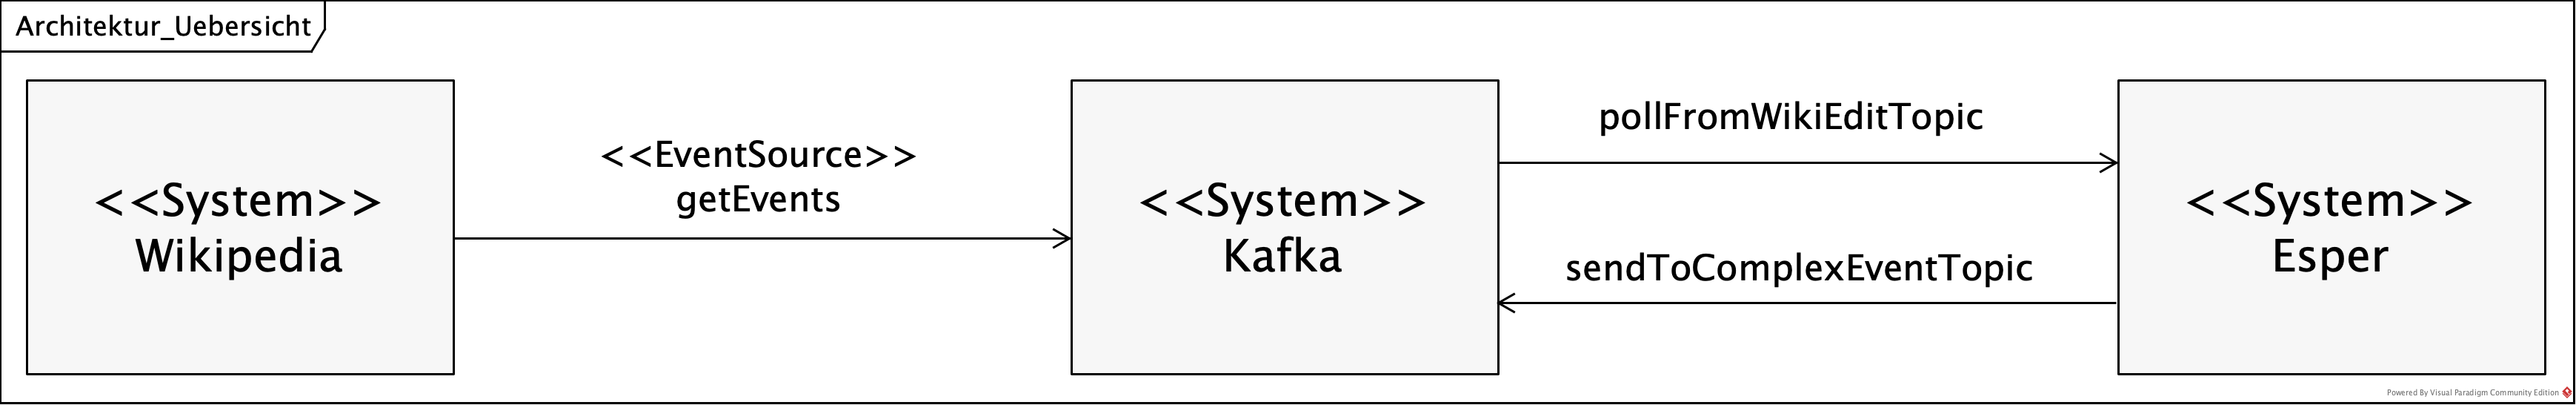
\includegraphics[width=\textwidth]{images/Architektur_Uebersicht.png}
    \caption{Architekturübersicht}
    \label{fig:architektur_uebersicht}
\end{figure*}

Abbildung \ref{fig:architektur_uebersicht} zeigt die Teilsysteme und deren Interaktion untereinander.

% Abbildung \ref{fig:architektur_uebersicht} zeigt bisher nur eine sehr rudimentäre Übersicht und soll als Grundlage dienen.
% Die Verbindung zwischen Esper und Kafka muss noch genauer werden: Protokoll, senden von komplexen Events in neue Kafka-Topics.

\subsection{Collection Tier: Wikipedia}
Wie zuvor beschrieben, stützt sich unser System auf Daten von Wikipedia. Wir nutzen den RecentChanges-Stream, der
Events zu neu erstellten, aktualisierten und gelöschten Wikipedia-Seiten enthält\footnote{https://www.mediawiki.org/wiki/Manual:RCFeed}.
Der Quellcode \ref{WikipediaRecentChangeJSON} zeigt einen Ausschnitt eines solchen Events.
Es sind nur die Attribut abgebildet, die in einem der nachfolgenden Teilsysteme relevant sind.

\begin{lstlisting}[label=WikipediaRecentChangeJSON,caption=Wikipedia RecentChange-Event,language=json,firstnumber=1,captionpos=b]
{
    "bot": false,
    "comment": "/* Politischer Werdegang */",
    "id": 269108829,
    "meta": {
        "uri": "https://de.wikipedia.org/wiki/Ingeborg_H%C3%A4ckel",
        "partition": 0,
        "offset": 1329388977
    },
    "timestamp": 1547910734,
    "title": "Ingeborg H\"ackel",
    "user": "Eszet2000",
    "wiki": "dewiki"
}
\end{lstlisting}

Die beiden Parameter \code{offset} und \code{uri}, innerhalb des \code{meta}-Objektes, stammen aus einem Kafka-System
und dienen der Wiederaufnahme eines abgebrochenen Streams. Wikipedia setzt intern Apache Kafka als Messaging-System ein.
Nach außen nutzt Wikipedia EventStreams. Das ist ein Webservice der kontinuierliche Datenströme mit strukturierten Daten
über HTTP sendet\footnote{https://wikitech.wikimedia.org/wiki/EventStreams}. Die Basis-Technologie dessen, ist
das Server-Sent Event (SSE) Protokoll. Der RecentChanges-Stream ist ein solcher Stream und kann über eine Client-Bibliothek
konsumiert werden.

Wie im vorherigen Kapitel beschrieben, werden Daten vom Collection Tier mithilfe eines der aufgelisteten Pattern übertragen.
SSE funktioniert nach dem One-way pattern, indem eine HTTP-Verbindung aufgemacht wird um Nachrichten zu empfangen \cite{EventSource_SSE}.

\subsection{Implementierungsdetails zum Messaging Queuing Tier: Kafka}
Im Messaging Queuing Tier setzen wir Apache Kafka in der Version 2.1 ein, um die im Collection Tier beschriebenen Wikipedia-Events
in unser eigenes Messaging-System zu überführen. Hierfür haben wir eine Java-Anwendung entwickelt, in der die folgenden
Schritte nacheinander ausgeführt werden:
\begin{enumerate}
    \item \textit{Kafka Initialisierung.} Den Host des Bootstrap-Servers setzen um eine Verbindung zu erzeugen.
    Als Key- und Value-Serialisierer setzen wir
    jeweils den \code{StringSerializer} von Kafka ein. Das heißt, die Events werden als JSON-String in das Topic \code{wikiEdit}
    eingespeist. Zum Senden von Events erzeugen wir ein Producer-Objekt mit dem passenden Typ \code{Producer<String, String>}.
    An dieser Stelle war die Überlegung, anstelle eines String-Serialisierers für den Wert des Producers,
    einen eigenen Serialisierer für die WikipediaEditEvent-Klasse einzusetzen. Wir entschieden uns aber für den
    String-Serialisierer, da Wikipedia die Events auch als JSON-String überträgt und wir in Kafka selbst
    keine weiteren Operationen an den Daten vornehmen. Eine mögliche Operation könnte ein Filter sein.
    Aber das einzige Ziel von Kafka soll die Persistierung und Weitergabe von Daten sein und dafür ist keine Serialisierung in
    einem bestimmten Typen notwendig. Außerdem verschiebt es Komplexität aus der Kafka-Anwendung
    in die Consumer-Anwendungen.
    \item \textit{Erzeugung eines EventHandlers.} Für das Empfangen von EventSource-Nachrichten nutzen wir die Java-Bibliothek
    \textit{okhttp-eventsource}\footnote{https://github.com/launchdarkly/okhttp-eventsource}. Zur Verarbeitung der Events
    \code{onOpen}, \code{onClose}, \code{onMessage}, \code{onComment} und \code{onError} muss das Interface \code{EventHandler} von
    \textit{okhttp-eventsource} implementiert werden.
    \item \textit{Erzeugung und Starten einer EventSource.} Mit der Stream-URI der Wikipedia-EventSource (für die RecentChanges ist das: https://stream.wikimedia.org/v2/stream/recentchange)
    und des implementierten EventHandler-Interfaces
    kann ein \code{EventSource}-Objekt erzeugt werden. Das Objekt dient dem Starten und Beenden eines EventSource-Streams.
    Die Daten werden dann, wie zuvor beschrieben, durch das SSE-Protokoll von Wikipedia an die Anwendung gesendet.
    \item \textit{Beim Eintreffen eines Events: Senden einer Nachricht in ein Kafka-Topic.} Tritt ein Wikipedia-Event auf,
    wird die \code{onMessage}-Methode des implementierten EventHandlers-Interface aufgerufen. Der zweite Parameter enthält die Daten
    des aufgetretenen Events. Der Zugriff auf die als JSON-String codierte Nachricht erfolgt über die \code{getDate()}-Methode.
    Diese Daten sendet die Anwendung, über den zuvor erzeugten Producer, ohne eine weitere
    Verarbeitung in das Kafka-Topic \code{wikiEdit}.
\end{enumerate}

Die Konfiguration der Kafka-Topics ist sehr einfach gehalten, da es sich bei der Anwendung nur um einen Prototypen handelt.
Wir haben ein Topic mit dem Namen \code{wikiEdit}. Da die Anwendung auf nur einem Server läuft, setzen wir auch nur
eine Partition ein und haben keine Replikation. Eine Skalierung der Kafka-Anwendung auf mehrere
parallel-arbeitende Server ist jedoch nicht ausgeschlossen für eine Produktivanwendung.

\subsection{Implementierungsdetails zum Analysis Tier: Esper}
In unserer Esper-Anwendung, die das Hauptsystem des Analysis Tier ist, nutzen wir Esper in Version 7.1
als Complex Event Processing-Werkzeug.
Zur Verarbeitung der Wikipedia-Events haben wir zwei Lösungen umgesetzt, da die erste Lösung nicht
zum Erreichen der Ziele führte. Für ein besseres Verständnis geben wir einen kurzen Überblick über den gemeinsamen Aufbau beider
Lösungen. Danach beschreiben wir die Details und Unterschiede der jeweiligen Lösungen und analysieren diese hinsichtlich der
Zielerfüllung.
In unserer Esper-Anwendung sind wir wie folgt vorgegangen:

\begin{enumerate}
    \item \textit{Esper Initialisierung.} Die Initialisierung von Esper besteht aus der Erzeugung einer \code{Configuration},
    der Erstellung und dem Starten von EPL-Statements, sowie dem Erzeugen von Listener-Klassen.
    \item \textit{Kafka initialisieren und starten.} Um die Daten aus dem Messaging Queuing Tier zu bekommen haben wir einen
    \code{KafkaConsumer<String, String>} implementiert.
    Wir pollen in einer Endlosschleife alle 10 Millisekunden die Daten vom Kafka-Topic \code{wikiEdit}. Bei den empfangenen Daten
    handelt es sich um einen String, der JSON enthält. Mithilfe der Gson-Bibliothek\footnote{https://github.com/google/gson}
    konvertieren wir die JSON-Strings in Java-Objekte. Die daraus resultierenden Java-Objekte senden wir wiederum in das
    Esper-System, damit darauf die EPL-Statements angewandt werden können.
    \item \textit{Aktion ausführen, sobald das Muster erfüllt ist.} Ist das Muster erfüllt, wird die \code{update}-Methode der Listener-Klasse
    aufgerufen. Es werden die alten und neuen Events übergeben. Daraus kann eine Aktion erfolgen, z.\,B. dass erzeugen eines neuen
    komplexen Events.
\end{enumerate}

Abbildung \ref{fig:class_diagram_eventtypes}


\begin{figure}[h]
    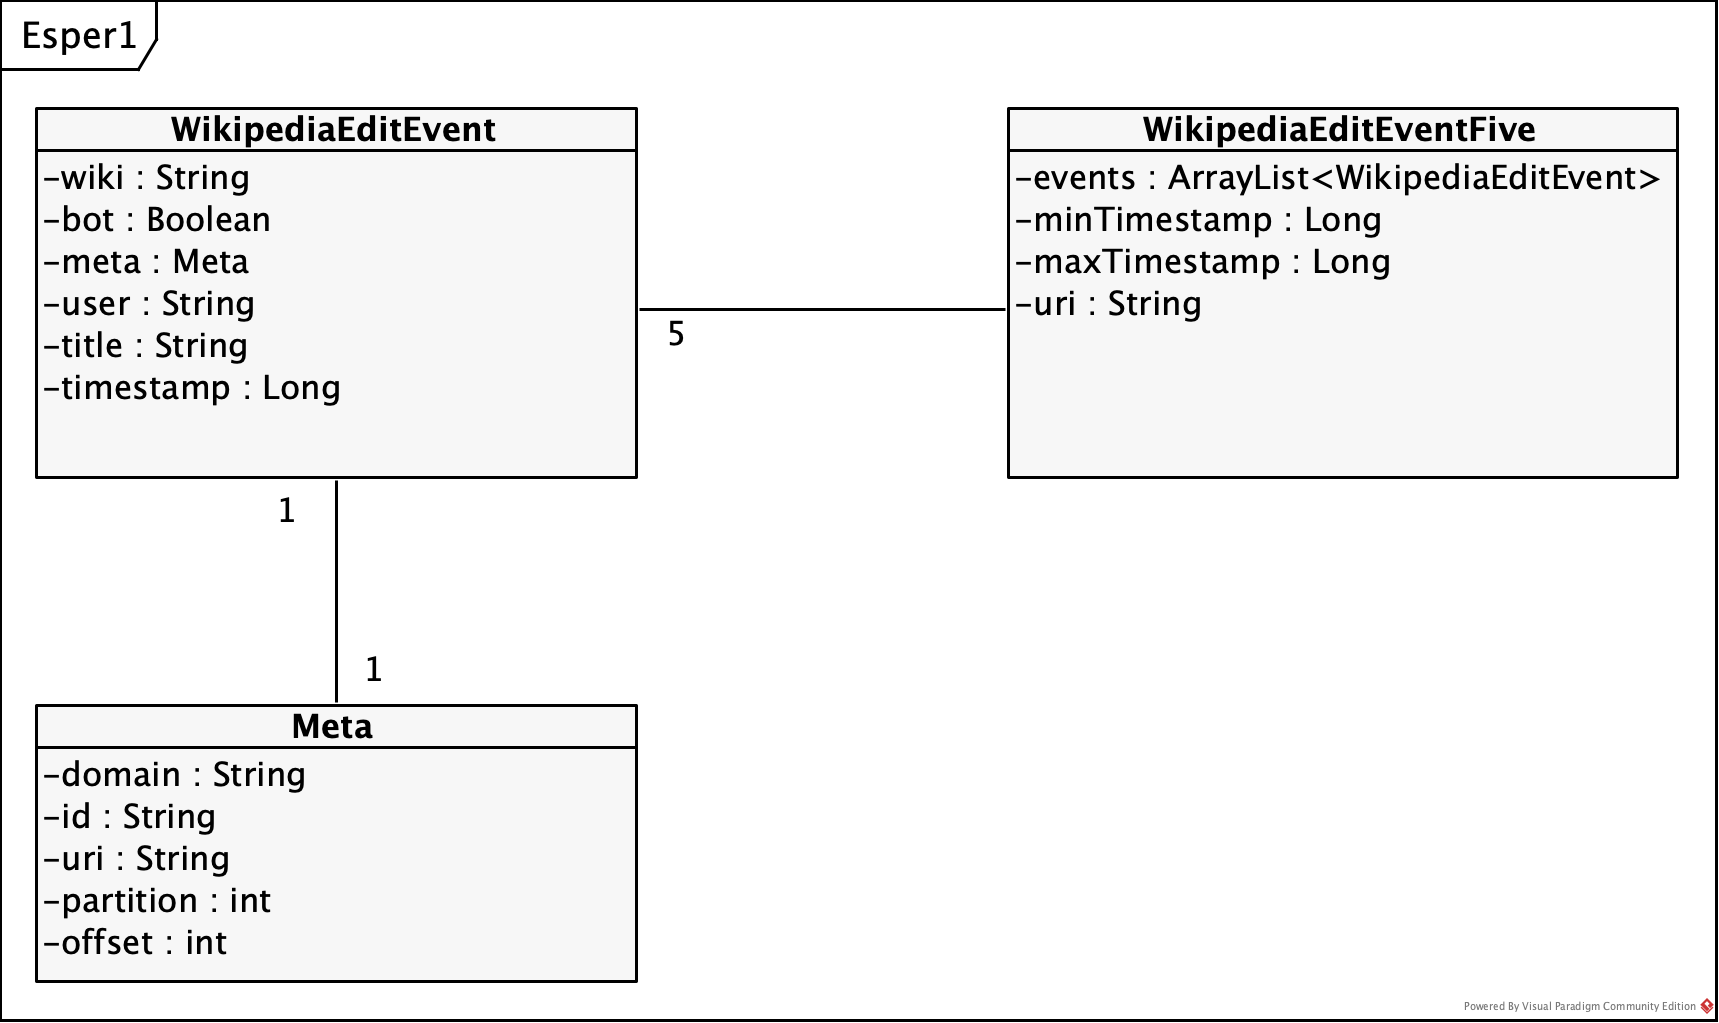
\includegraphics[width=.5\textwidth]{images/Esper1.png}
    \caption{Klassendiagramm der zwei Ereignistypen WikipediaEditEvent, WikipediaEditEventFive und der Helferklasse Meta}
    \label{fig:class_diagram_eventtypes}
\end{figure}


Genaueres zu den erzeugten Expressions im nächsten Kapitel.

Einsatz von GSON

\subsection{BurstDetection-Implementierung}